\documentclass[uplatex,dvipdfmx,a4paper,11pt]{jsarticle}

\usepackage{amsmath,amsthm,amssymb}
\usepackage[dvipdfmx]{graphicx}
\usepackage{bm}
\usepackage{ascmac}
%
\usepackage{multirow}
\usepackage{wrapfig}
%
\pagestyle{empty}
%% 高さの設定
\setlength{\textheight}{\paperheight}   % ひとまず紙面を本文領域に
\setlength{\topmargin}{-5.4truemm}      % 上の余白を20mm(=1inch-5.4mm)に
\addtolength{\topmargin}{-\headheight}  % 
\addtolength{\topmargin}{-\headsep}     % ヘッダの分だけ本文領域を移動させる
\addtolength{\textheight}{-40truemm}    % 下の余白も20mmに%% 幅の設定
\setlength{\textwidth}{\paperwidth}     % ひとまず紙面を本文領域に
\setlength{\oddsidemargin}{-5.4truemm}  % 左の余白を20mm(=1inch-5.4mm)に
\setlength{\evensidemargin}{-5.4truemm} % 
\addtolength{\textwidth}{-40truemm}     % 右の余白も20mmに

%
\abovecaptionskip=-1pt
%\belowcaptionskip=-1pt
%
\renewcommand{\baselinestretch}{0.9} % 全体の行間調整
\renewcommand{\figurename}{Fig.}
\renewcommand{\tablename}{Tab.}
%
\makeatletter 
\def\section{\@startsection {section}{1}{\z@}{1.5 ex plus 2ex minus -.2ex}{0.5 ex plus .2ex}{\large\bf}}
\def\subsection{\@startsection{subsection}{2}{\z@}{0.2\Cvs \@plus.5\Cdp \@minus.2\Cdp}{0.1\Cvs \@plus.3\Cdp}{\reset@font\normalsize\bfseries}}
\makeatother 
%
\graphicspath{{../../figures//}}
%
\begin{document}

%%%%%%
% はじめに
%%%%%%
\begin{center}
{\Large \textgt{22. ランダム構造を有するネットワークポリマーの緩和挙動}}
\end{center}

\begin{flushright}
東亞合成 佐々木裕

Tel: 052-611-9923, e-mail: hiroshi\_sasaki$@$mail.toagosei.co.jp
\end{flushright}

\vspace{0.5\baselineskip}
\section{はじめに}

ゴムの大きな破壊靭性の由来については、 ヒステリシスロスのようなエネルギー散逸により亀裂進展が抑制されるという Andrews モデルが提案されている~\cite{Andrews1977}。
ゴムへのフィラーの添加がヒステリシスの主要な発生原因とされ~\cite{Grosch1968}、その発現機構の一つとしてフィラー近傍でのナノキャビティーの開閉も報告されている~\cite{Zhang2013}。
フィラー由来の靭性向上効果はメゾスケール領域の挙動であると考えられているが、このようなエネルギー散逸挙動はメゾスケールでしか発現しないのであろうか?

ゴム弾性の古典的なモデルは、ガウス鎖をストランドとしたとネットワークの結節点のミクロな変形がマクロな変形と相似でアフィン変形するとした``Affine Network Model: ANM'' である。%~\cite{Flory1953}。
この古典モデルからの発展形として、結節点の揺らぎに注目しミクロな変形がマクロと異なるとした``Phantom Network Model: PNM''が提案され~\cite{James1943}、Flory によれば、メルト状態と同一なストランドのゆらぎを有するランダムネットワークにおいて PNM のふるまいを示すとされている~\cite{Flory1976}。
我々は、この結節点のゆらぎ由来の散逸が、分子鎖描像のようなミクロなスケールでの粘弾性的なエネルギー散逸モデルとなりうるのではないかと考えている。

我々は、規則構造ネットワークをベースとしてユニットセル間における規則性をランダムへと変えることで架橋欠損のないネットワークを作成して PNM を再現できる系の構築を目指し、「スヌケ鎖」での再現については昨年のこの会にて報告した。
本報告では、「KG鎖」への拡張を検討した結果について報告する。

\section{シミュレーション}

\subsection{ネットワークモデルの作成}

任意の分岐数$f$($f=3\sim6$)の結節点からなる規則構造を有するネットワークに対して、トポロジーモデルの「代数的連結性」を指標として以下のアルゴリズムでランダムな結合性を導入した。
% \vspace{-2mm}
\begin{enumerate}
\item
実空間で"8-Strand Unit Cell"の周期境界での連なり(2x2x2=8 Cells)の初期構造を作成(Fig. \ref{fig:cells})。
\item
初期構造に対応したトポロジーモデルを用いてノードごとのエッジ数(分岐数)に変換(Fig. \ref{fig:topo})。
\item
トポロジーモデルにて、ネットワークの結びつきの強さを表す代数的連結性を指標として連結性を維持しながらストランド交換し、結節点の結合性にランダム性を導入(Fig. \ref{fig:exc})。
\item
そのトポロジーモデルに対応するように、実空間の初期構造からストランドを除去。
\end{enumerate}

\begin{figure}[hb]
\begin{minipage}{0.33\hsize}
	\begin{center}
	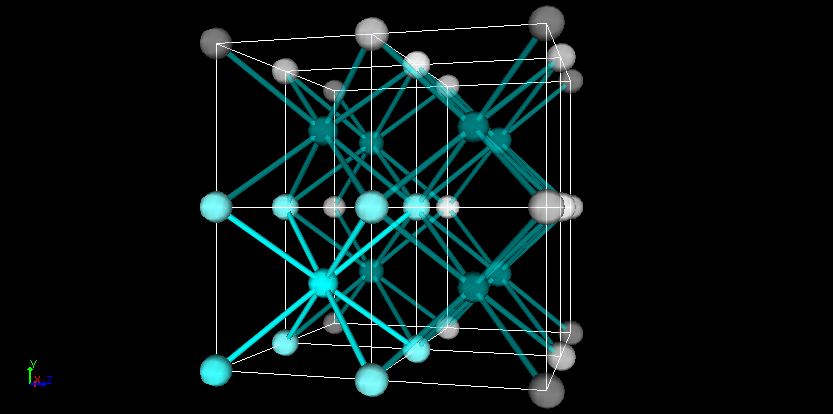
\includegraphics[width=50mm]{8_per.png}
	\caption{$2^3$ of 8-Strand Unit Cells}
	\label{fig:cells}
	\end{center}
\end{minipage}
\begin{minipage}{0.33\hsize}
	\begin{center}
	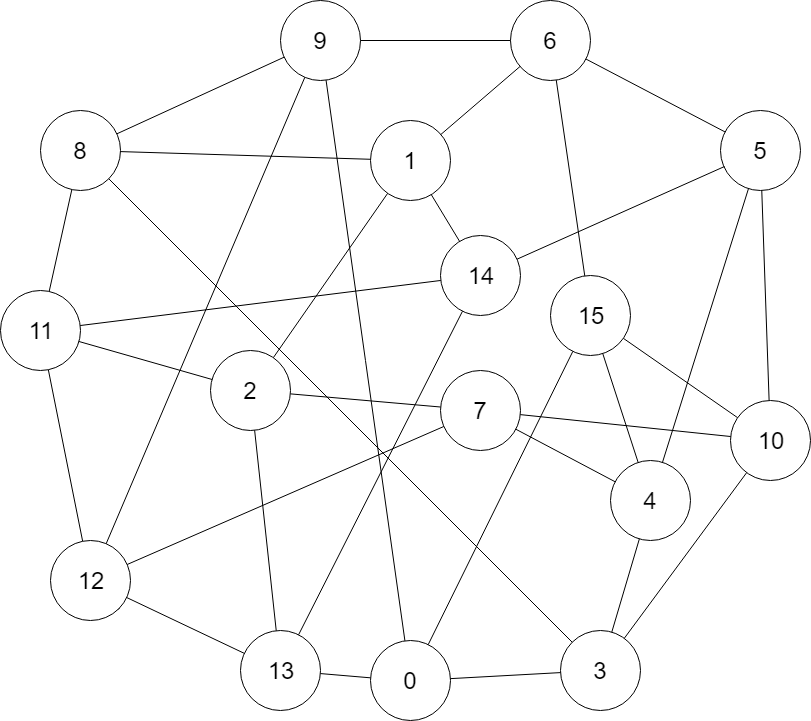
\includegraphics[width=30mm]{Network.png}
	\caption{Topological NW Model}
	\label{fig:topo}
	\end{center}
\end{minipage}
\begin{minipage}{0.33\hsize}
	\begin{center}
	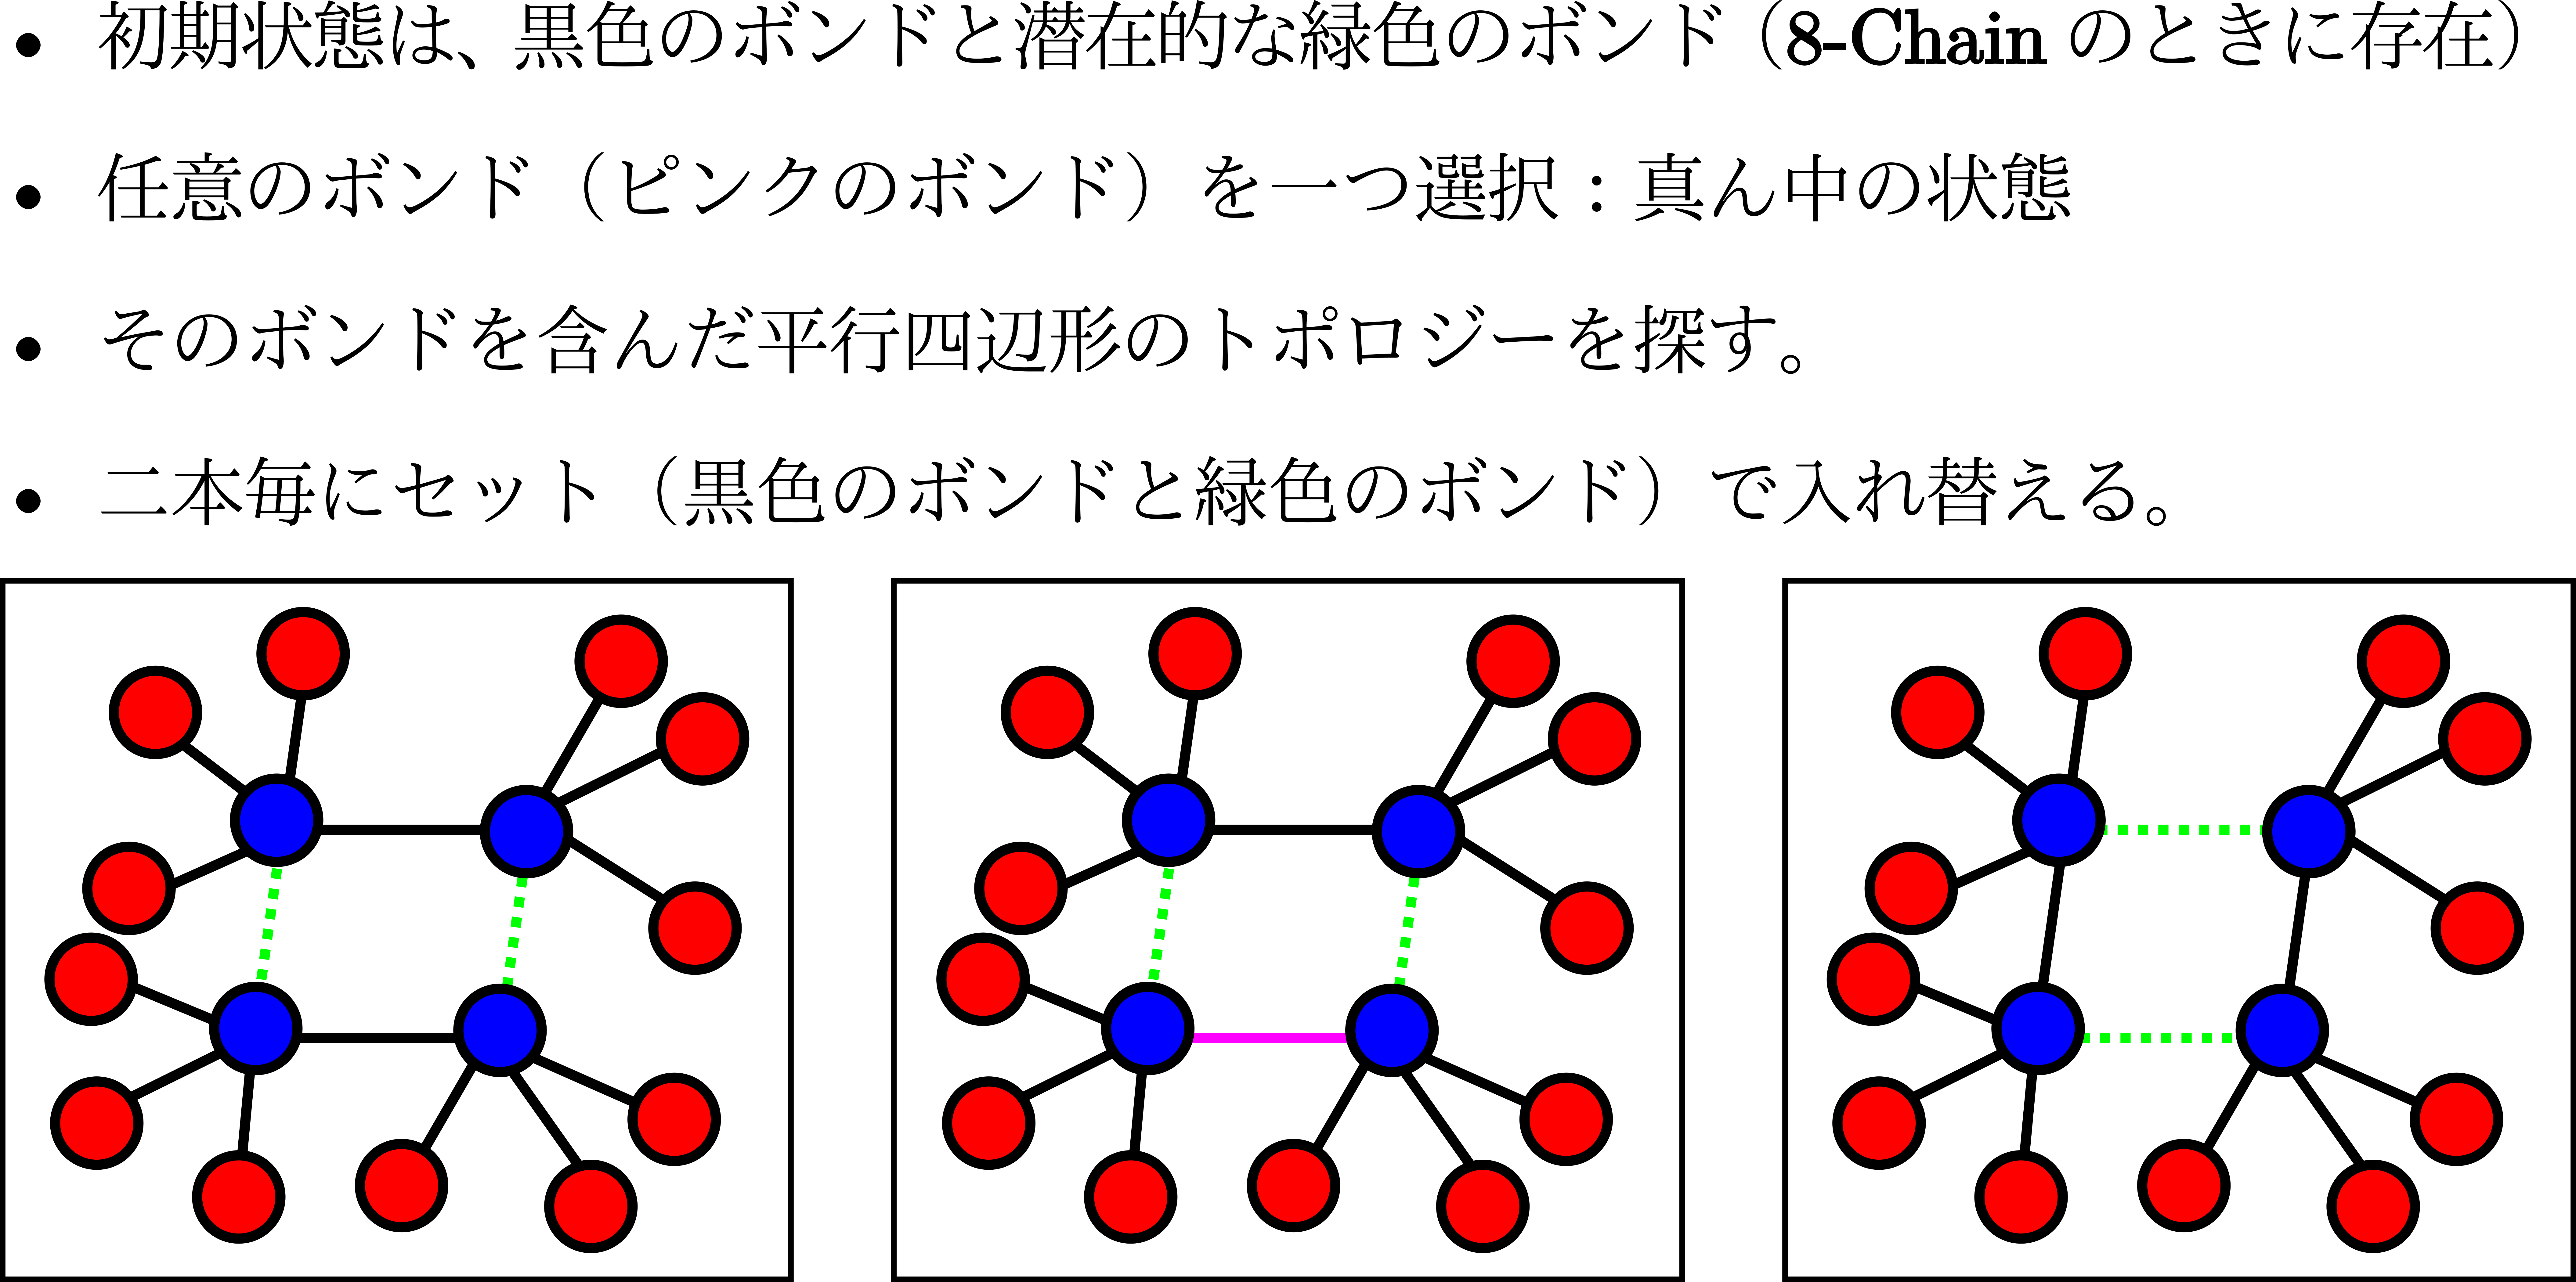
\includegraphics[width=50mm]{bond_exchg.png}
	\caption{Strand Exchange Procedure}
	\label{fig:exc}
	\end{center}
\end{minipage}
\end{figure}

\subsection{MD シミュレーション}

上記にて生成したランダムな結合性を有するネットワークを初期構造として、OCTA 上の COGNAC シミュレーターにより MD シミュレーションを行った。
ユニットセル中でのストランドの末端間距離がホモポリマーと同等になるようにストランド長と多重度を調整し、緩和計算により平衡構造を得た。


非結合ポテンシャルは LJ ポテンシャル $U_{LJ}(r_{ij})$によりビーズ間に斥力相互作用($r_c = 2^{(1/6)}\sigma$)を、また、ボンドポテンシャルには FENE-LJ ポテンシャルを用いて KG 鎖とした。
なお、初期構造の緩和は、Auhl 等の方法~\cite{Auhl2003a} に従い、force-capped-LJ ポテンシャルを用いた Slow Push Off により行った。
また、密度の低い初期状態から NPT 計算により圧縮することで、絡み合いを極力排除した比較計算も実施した。
% \begin{figure}[htb]
    \begin{center}
        \begin{minipage}{0.46\textwidth}
            \begin{itembox}[l]{KG 鎖で用いるポテンシャル}
                \scriptsize
                \begin{align*}
                    &U_{LJ}( r_{ij} ) =
                    \begin{cases}
                    4\epsilon_{LJ} \left[ \left( \dfrac{ \sigma }{ r_{ij} } \right)^{12} - \left( \dfrac{ \sigma }{ r_{ij} } \right)^{6} \right] \; & r_{ij}< r_c \\[8pt]
                    0 \; & r_{ij} \geq r_c
                    \end{cases} \\[10pt]
                    &U_{FENE}( r ) = 
                    \begin{cases}
                    -\dfrac{1}{2} k R_0^2 \ln \left[ 1 - \left( \dfrac{ r }{ R_0 } \right)^{2} \right]  \; & r < R_0 \\[8pt]
                    \infty \; & r \geq R_0
                    \end{cases} \\[8pt]
                    &\; where \; R_0 = 1.5 \sigma, k = 30 \notag
                    \end{align*}
            \end{itembox}
        \end{minipage}
        \begin{minipage}{0.5\textwidth}
            \begin{itembox}[l]{Slow Push Off のためのポテンシャル}
                % force-capped-LJ ポテンシャル
                \scriptsize
                \begin{align*}
                    &U_{FCLJ}(r) = 
                    \begin{cases}
                    (r-r_{fc})*U_{LJ}^{\prime}(r_{fc}) + U_{LJ}(r_{fc}) \;\;\; &r< r_{fc} \\[8pt]
                    U_{LJ}   \;\;\;\;\;\;\;\;\; &r \geq r_{fc}
                    \end{cases} \\[10pt]
                % \end{align*}
                % % ボンドポテンシャル
                % \begin{align*}
                    &U_{bond}(r) = 20.2026 \varepsilon + 490.628 \varepsilon \left(\dfrac{r-r_0}{\sigma}\right)^2 \\[8pt]
                    & \;\;\;\;\;\;\;\;\;\;\;\;\;\;\;\;\;\;  - 2256.76 \varepsilon \left(\dfrac{r-r_0}{\sigma}\right)^3 + 9685.31  \varepsilon \left(\dfrac{r-r_0}{\sigma}\right)^4
                    \end{align*}
            \end{itembox}
            % \begin{center}
            % \includegraphics[width=\textwidth]{.png}
            % \end{center}
        \end{minipage}
        % \vspace{3mm}
        % \caption{Non-bond and Bond Potentioals used for MD simulations by Cognac on OCTA}
        % \label{}
    \end{center}
% \end{figure}

\section{結果と考察}
セグメント数 N=48 のストランドを選択し多重度を変えることで同様な鎖密度 $\nu$ を有する三、四分岐モデル(多重度はそれぞれ 4 と 3、3 or 4-Chainと表記)を作成し、シミュレーションを行った。

\subsection{ストランドのセグメント間距離 $\langle \bm{R} \rangle$ の分布関数}

四分岐モデルにおけるストランドの長手方向に沿ったセグメント間距離($n=48$ で末端間距離に対応)の分布関数のトラジェクトリーを、ホモポリマーの平均値とともに Fig.\ref{fig:e2e} に示した。
部分鎖としての振る舞いは拘束のないメルトポリマー鎖と類似であったが、そのゆらぎは若干低下していた。

\subsection{$\lambda =2$ からの応力緩和}
システムの鎖密度を同一としたネットワークを $\lambda =2$ まで迅速に伸長し、応力緩和関数 $G(t)$ を求めた (Fig.\ref{fig:stress_rel})。
緩和後の弾性率は三分岐の方が低くなったが、いずれも ANM よりも高かった。
これは Trapped Entanglement により実効的な鎖密度が上昇したと考えられたため、Primitive Path Analysis (PPA) を行い、多数の絡み合いを確認した (Fig.\ref{fig:ppa})。
また、NPT 計算により絡み合いを排除した比較 (4-Chain-NPT) では PPA にて絡み合いが殆どないことが確認でき、弾性率が PNM へと漸近していた。

\begin{figure}[hb]
\begin{minipage}{0.34\hsize}
    \begin{center}
        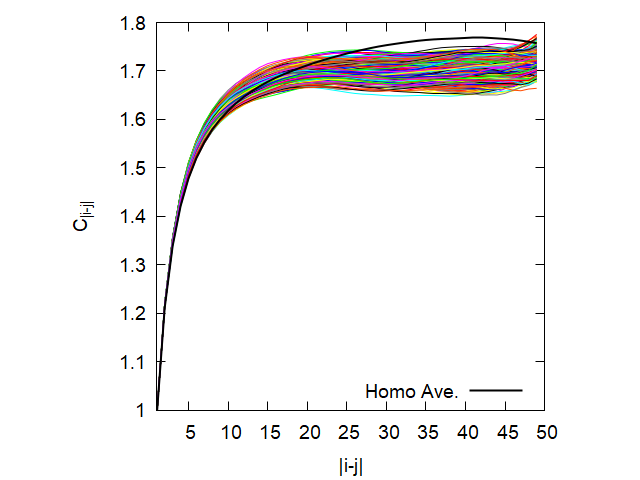
\includegraphics[width=\textwidth]{N48_f4_CN.png}
	    \caption{Trajectry of Mean Square Internal Distance distribution of strands for 4-Chain Model}
	    \label{fig:e2e}
	\end{center}
\end{minipage}
\begin{minipage}{0.34\hsize}
	\begin{center}
		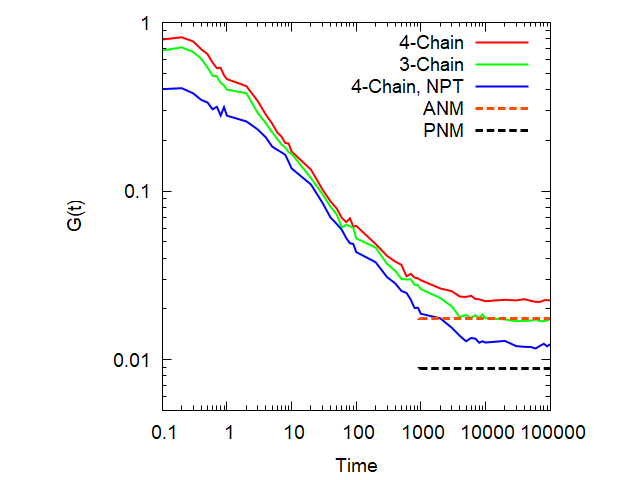
\includegraphics[width=\textwidth]{gt_comp_34.png}
        \caption{Stress Relaxations for Uni-axial Step Strain($\lambda=2$)}
        \label{fig:stress_rel}
	\end{center}
\end{minipage}
\begin{minipage}{0.32\hsize}
	\begin{center}
		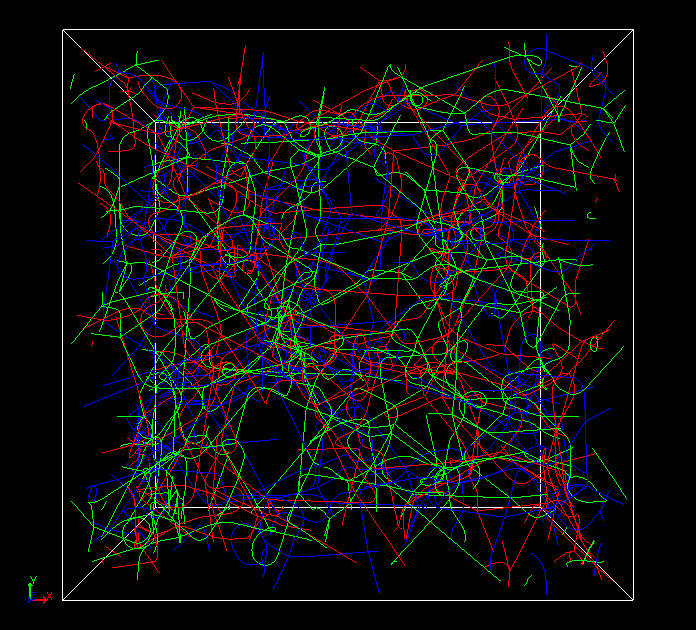
\includegraphics[width=.8\textwidth]{N48_f4_PPA.png}
        \caption{Primitive Path Analysis (PPA) for 4-Chain Model}
        \label{fig:ppa}
	\end{center}
\end{minipage}
\end{figure}

\vspace{-3mm}

\bibliographystyle{../achemso}
\bibliography{D:/Dropbox/Bibliography/library.bib}

\end{document}